
We followed the standard evaluation procedure for the WebQuestions dataset and used the original 70-30\% train-test split, which results in 3,778 training and 2,032 test questions.
Since each answer is potentially a list of entities $a^*$, the quality of an answer $a$ is represented by F1-score: 
$$f1(a^*, a) = 2\frac{precision(a^*,a) recall(a^*,a)}{precision(a^*,a) + recall(a^*,a)}$$
where $precision(a^*, a)=\frac{|a^* \cap a|}{|a|}$ and $recall(a^*, a) = \frac{|a^* \cap a|}{|a^*|}$.

We also report average precision and recall, as well as an F1 score of average precision and recall.
The results of existing approaches, our baseline and Text2KB systems is presented in Table \ref{table:webquestions_results}.

\begin{table*}
\centering
\caption{Performance of the Text2KB system on WebQuestions dataset compared to the existing approaches. The difference from the baseline Aqqu system is significant with p-value < 0.01}
\label{table:webquestions_results}
\begin{tabular}{| p{5cm} | p{1.5cm} | p{1.5cm} | p{1.5cm} | p{1.5cm} | }
\hline
System & avg Recall & avg Precision & F1 of avg Prec and Recall & avg F1 \\
\hline
SemPre \cite{Berant:EMNLP13} & 0.413 & 0.480 & 0.444 & 0.357\\
Subgraph Embeddings \cite{BordesCW14:emnlp} & - & - & 0.432 & 0.392\\
ParaSemPre \cite{berant2014semantic} & 0.466 & 0.405 & 0.433 & 0.399\\
Jacana \cite{yao2014information} & 0.458 & 0.517 & 0.486 & 0.330\\
Kitt AI \cite{yao-scratch-qa-naacl2015} & 0.545 & 0.526 & 0.535 & 0.443\\
AgendaIL \cite{berant2015imitation} & 0.557 & 0.505 & 0.530 & 0.497\\
STAGG \cite{yih2015semantic} & \textbf{0.607} & \textbf{0.528} & \textbf{0.565} & \textbf{0.525}\\
% STAGG (no duplicates\footnote{An answer of the STAGG system may contain duplicate entities, which are double counted by the evaluation script}) \cite{yih2015semantic} & 0.6067 & 0.5263 & 0.5634 & 0.5234 \\
\hline
Aqqu (baseline) \cite{ACCU:2015} & 0.604 & 0.498 & 0.546 & 0.494\\
% DIDN'T HAVE TIME TO IMPLEMENT THIS.
% Text-only baseline & & & & \\
Our system: Text2KB & 0.6354 & 0.5059 & 0.5633 & 0.5223 \\
\hline
\end{tabular}
\end{table*}

As we can see, Text2KB significantly improves over the baseline system and reaches the current best published result - STAGG \cite{yih2015semantic}, and we believe that this system will also benefit from the ideas of our work, and we will explore this question in Section \ref{section:analysis}.

\subsection{Ablation Study}

To study effects of different components in isolation we made a series of ablation studies.
For convenience, we introduce the following notations for different components of our system:
\vspace{-0.1cm}
\begin{itemize}
\setlength\itemsep{-0.5em}
\item T - notable type score model as a ranking feature
\item DF - date range filter-based query template
% \item TF - using notable type based filter
\item E - using web search result snippets for question entity identification
\item W - using web search results for feature generation
\item CQA - using CQA-based \texttt{[question term, KB predicate]} PMI scores for feature generation
\item CW - features, computed from entity pairs language model, estimated on ClueWeb
\end{itemize}

In our results table we will use the notation \texttt{+$<$component$>$} to for a system with a certain component added, and \texttt{-$<$component$>$} when the component is removed.
For example, the baseline system will be denoted as ``\texttt{Aqqu}'' according the authors notation.
The same system with additional date range filter query templates and notable types score model is denoted as ``\texttt{Aqqu +DF+T}'', which represents the same system as ``\texttt{Text2KB -E-W-CQA-CL}''.
Our full system ``\texttt{Text2KB}'' can be also denoted as ``\texttt{Aqqu +DF+T+E+W+CQA+CL}''.

\begin{table}
\caption{Average Recall (R), Precision (Pr), and F1 of Aqqu (baseline), Text2KB (our system), and variations of TextKB with respective components removed. * indicates significant differences at p<0.05. }
\label{table:ablation:entities_vs_features}
\begin{tabular}{| p{4.2cm} | c | c | c | }
\hline
System & R & Pr & F1 \\
\hline
% THIS TELLS HOW MUCH EXTERNAL ENTITIES GIVE COMPARED TO MY OTHER IMPROVEMENTS
\texttt{Aqqu} (baseline) & 0.604 & 0.498 & 0.494\\
% baseline_typemodel_dates.log : baseline with types model +dates, but without any text-based data
\texttt{Text2KB -E-W-CQA-CL}= =\texttt{Aqqu +DF+T} & 0.6169 & 0.4807 & 0.4987 \\
% extent_dates_typemodel_rf100.log : -web-cqa-clueweb
\texttt{Text2KB -W-CQA-CL} & 0.6272* & 0.4920* & 0.5083* \\  % AND FEATURES GIVE THE REST
% web_cqa_clueweb_typemodel_dates.log : -external entities (Text features on top my other improvements)
\texttt{Text2KB -E} & 0.6344* & 0.4966* & 0.5140* \\  % AND FEATURES GIVE THE REST
%\hline
% extent_web_cqa_clueweb_dates_types_typemodel_rf100.log : everything, including type filters
%\texttt{Text2KB} & 0.6354* & 0.5059* & 0.5223* \\
\hline
\end{tabular}
\end{table}

The first question that we are asking is what are the improvements, introduced by adding date range filter templates, notable type model, entity linking from web search results and text-based features generated from all the different sources.
Results of this ablation experiment are presented in Table \ref{table:ablation:entities_vs_features}.
As we can see, additional date range filters and notable types model (\texttt{Text2KB -E-W-CQA-CL}) are responsible for an increased recall and a drop in precision compared to the baseline model.
Detecting question entities (\texttt{Text2KB -W-CQA-CL}) help improve both precision and recall, and therefore average F1 score by 0.096 points.
An even bigger improvement is achieved by introducing all our external text-based features, and since these improvements are independent, their combination boosts the performance even more.

Now, let's look into the relative importance of each of the data sources, we will remove or use a group of web search, cqa or clueweb-based features and see how the performance of the whole system changes.
Table \ref{table:ablation:features} summarizes the results of these experiments.

\begin{table}
\caption{Average Recall (R), Precision (Pr), and F1 of Text2KB variations with and without features based on web search results, CQA data and ClueWeb collection}
\label{table:ablation:features}
\begin{tabular}{| p{4cm} | c | c | c | }
\hline
System & R & Pr &  F1 \\
\hline
% THIS PART ANSWERS HOW GOOD ARE EACH OF THE PROPOSED DATASETS
% extent_cqa_clueweb_dates_typemodel_rf100.log : -web
\texttt{Text2KB -W} & 0.6327 & 0.4960 & 0.5126 \\
% extent_web_clueweb_dates_typemodel_rf100.log : -cqa
\texttt{Text2KB -CQA} & 0.6420 & 0.4987 & 0.5185 \\
% extent_web_cqa_dates_typemodel_rf100.log : -clueweb
\texttt{Text2KB -CL} & 0.6444 & 0.5047 & 0.5228 \\
\hline
% extent_web_dates_typemodel_rf100.log : -clueweb-cqa
\texttt{Text2KB} (Web search results only) & 0.6423 & 0.5028 & 0.5216 \\
% extent_clue_dates_typemodel_rf100.log : -web-cqa
\texttt{Text2KB} (ClueWeb only) & 0.6307 & 0.4978 & 0.5138 \\
% extent_cqa_dates_typemodel_rf100.log : -web-clueweb
\texttt{Text2KB} (CQA only) & 0.6224 & 0.4928 & 0.5077 \\
%\hline
% extent_web_cqa_clueweb_dates_types_typemodel_rf100.log : everything, including type filters
%\texttt{Text2KB} & 0.6354 & 0.5059 & 0.5223 \\
\hline
\end{tabular}
\end{table}

Features that we generate from web search results are the most effective, because even without other data sources the QA performance is almost as high as the full system.
In addition, if we remove web search results based features the performance drops more than for other text data sources.
Features based on ClueWeb entity pair statistics perform better than CQA-based features.

% THIS EXPERIMENTS ARE REDUNDANT
%\begin{table}
%\caption{Evaluation study for our system with different text-based data sources used to generate features}
%\label{table:ablation:other}
%\begin{tabular}{| p{4cm} | c | c | c | }
%\hline
%System & avg Re & avg Pr &  avg F1 \\
%\hline
%AQQU & 0.604 & 0.498 & 0.494\\
%Text2KB -TF & 0.6429 & 0.5030 & 0.5220 \\
%\hline
% THIS PART SHOULD ANSWER HOW TEXT BASED FEATURED COMPARE TO EXTERNAL ENTITIES
% web_cqa_clueweb_typemodel_rf100.log : web+cqa+clueweb+typemodel -external-dates
%Text2KB +W+CQA+CW+T-E & 0.6351 & 0.4933 & 0.5104 \\
% web_cqa_clueweb_noext_rf100.log : web+cqa+clueweb -external-dates-typemodel
%Text2KB +W+CQA+CW-E & 0.6414 & 0.4981 & 0.5160 \\
% typemodel_rf100.log : type model only
%Text2KB +T-W-CQA-CL-E & 0.6131 & 0.4747 & 0.4918 \\
%\hline
%\end{tabular}
%\end{table}

Since we used each data source to generate multiple different features for candidate ranking, it is interesting to see which particular features are  more useful than others by the ranking machine learning algorithm (we used random forest).
Figure \ref{fig:feature_importances} plots a subset of features ranked by their Gini index-based importance scores in the final answer candidate ranking model.

\begin{figure*}
\centering
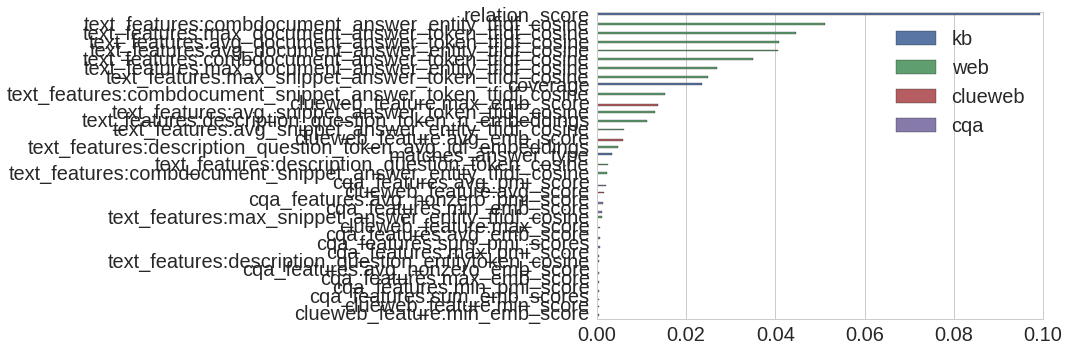
\includegraphics[width=0.9\textwidth]{img/feature_importances}
\vspace{-0.5cm}
\caption{Importances of different text-based features for KBQA (features with * are not text-based and are provided for comparison)}
\label{fig:feature_importances}
\end{figure*}

The figure supports the observation that web search results features are the most useful, however, other text data sources also contribute to the improvement.

In summary, Text2KB significantly outperforms the baseline system, and each of the introduced components contributes to this improvement.
Web search results data turned out to be the most useful resource, and it significantly improves the quality by helping with question entity identification and candidate ranking.
Next, we analyze the system performance in more detail, and investigate factors for future extension.